% inspired from: https://github.com/SnipyJulmy/hesso-latextemplate-lab
\documentclass[11pt,a4paper,oneside]{report}
\usepackage[margin=2cm]{geometry}
\usepackage[utf8]{inputenc}
\usepackage[T1]{fontenc}
\usepackage[french]{babel}
\usepackage{minted}
\usepackage{titlesec}
\usepackage[pdftex]{graphicx} % graphics importing
\usepackage{titling} % can use \theauthor \thetitle
\usepackage{parskip} % remove first line indenting in a section
\usepackage{microtype} % typographic improvements
\usepackage[defaultlines=3,all]{nowidow}
\usepackage[toc,page]{appendix}
\usepackage{verbatim}
\usepackage{float}

% Header and Footer
\usepackage{fancyhdr}

% style for all normal pages
\fancypagestyle{normal}{
\fancyhf{}
\setlength\headheight{14pt}
\lhead[]{Docker and Embedded systems}
\chead[]{}
\rhead{
\includegraphics[width=3cm]{img/mse_logo}}
\cfoot[]{\thepage}
\renewcommand{\headrulewidth}{0.4pt}% Default \headrulewidth is 0.4pt
\renewcommand{\footrulewidth}{0.4pt}% default is 0pt
}

% style for history
\fancypagestyle{historystyle}{
\setlength\headheight{14pt}
\lhead[]{Docker and Embedded systems}
\chead[]{}
\rhead{
\includegraphics[width=3cm]{img/mse_logo}}
\renewcommand{\headrulewidth}{0.4pt}% Default \headrulewidth is 0.4pt
\renewcommand{\footrulewidth}{0pt}
}

\usepackage[hyphens]{url} % line wrap urls
\usepackage{hyperref}

% Version history
\usepackage{vhistory}

\newminted{bash}{xleftmargin=20pt, linenos=true, breaklines=true, frame=single, framesep=6pt, tabsize=2, fontfamily=courier, fontsize=\small}

% Chapter titles
% Remove space before title
\titlespacing{\chapter}{0pt}{*-4}{*3}
% Remove "Chapter N" and use a sans-serif font
\titleformat{\chapter}{\normalfont\huge}{\thechapter.}{20pt}{\huge}
% Change chapter page style
\patchcmd{\chapter}{plain}{fancy}{}{}

\newcommand{\code}[1]{\texttt{#1}} % inline code

\title{État de l'art à la mi-projet de semestre Docker and embedded systems - Ou comment ne pas cross compiler Docker sur ARM}
\author{Gary \bsc{Marigliano}}

\begin{document}

\begin{titlepage}
\begin{center}


\includegraphics[width=0.6\textwidth]{img/docker_logo}\\[1cm]

\begin{figure}[htbp]
\begin{minipage}[c]{.45\linewidth}
\begin{flushleft}

\includegraphics[width=7cm]{img/mse_logo}
\end{flushleft}
\end{minipage}
\hfill
\begin{minipage}[c]{.45\linewidth}
\begin{flushright}

\includegraphics[height=2cm]{img/logo_hes-so}
\end{flushright}
\end{minipage}
\end{figure}

% Title
\rule{\linewidth}{0.5mm} \\[0.4cm]
{ \huge \bfseries \thetitle \\[0.4cm] }
\rule{\linewidth}{0.5mm} \\[1.5cm]

% Author and supervisor
\noindent
\begin{minipage}{0.4\textwidth}
  \begin{flushleft} \large
    \emph{Auteur :}\\
    \theauthor
  \end{flushleft}
\end{minipage}%
\begin{minipage}{0.4\textwidth}
  \begin{flushright} \large
    \emph{Encadrant :} \\
    Jean-Roland \bsc{Schüler}
  \end{flushright}
\end{minipage}

\vfill

\noindent
\begin{minipage}{0.4\textwidth}
  \begin{flushleft} \large
    \emph{Contact :}\\
    gary.marigliano@master.hes-so.ch
  \end{flushleft}
\end{minipage}%
\begin{minipage}{0.4\textwidth}
  \begin{flushright} \large
    \emph{Mandant :} \\
    Haute école d'ingénierie et d'architecture de Fribourg
  \end{flushright}
\end{minipage}

\vfill

% Bottom of the page
{\large Version 0.0.2 \\ \today}

\end{center}
\end{titlepage}

\pagestyle{historystyle}
\begin{versionhistory}  
  \vhEntry{0.0.1}{15.04.16}{\theauthor}{Création du document}
  \vhEntry{0.0.2}{01.05.16}{\theauthor}{Modifications première page, ajout historique, repositionnement des images}
\end{versionhistory}


\pagenumbering{gobble}
\tableofcontents
\pagenumbering{arabic}

\pagestyle{normal}

\chapter{Introduction}

\section{Contexte}\label{contexte}

Ce document s'inscrit dans le cadre du projet de semestre Docker and embedded systems actuellement réalisé par moi-même. Un des buts de ce projet est de cross compiler Docker à partir de ses sources pour produire un binaire exécutable sur un Odroid XU3 (ARMv7).

Lien: \url{https://github.com/krypty/docker_and_embedded_systems}

Il est important de noter que la vitesse de développement de Docker est assez hallucinante. En effet, sur Github (\url{https://github.com/docker/docker}) les commits se succèdent à vitesse grand V. Entre chaque version de Docker qui sortent environ tous les mois, il est courant d'avoir plus de 3000 commits qui ont été \emph{pushés}. Tout ceci pour dire qu'à la lecture de ce document, il est quasiment sûr que certaines pistes explorées soient définitivement obsolètes ou au contraire deviennent la voie à suivre du à une mise à jour quelconque.


\section{Objectifs}

De manière plus précise, ce projet vise à maitriser les parties suivantes:

\begin{enumerate}
  \item Construction d'un système Linux capable de faire tourner Docker et son \emph{daemon} en utilisant Buildroot. Pour générer le dit système, on dispose d'un \emph{repository} Gitlab hébergé à la Haute École de Fribourg

  \item Cross compilation de Docker et de son \emph{daemon}, capable de faire tourner des containers
\end{enumerate}

L'objectif de ce document est d'énumérer les différentes techniques tentées pour (cross-)compiler Docker sur une cible ARM. De cette manière, le lecteur, en cas de reprise du projet ou par simple curiosité, aura une idée des pistes à explorer ou à éviter.



\chapter{Objectif 1 - Construction d'un système GNU/Linux Docker-ready}

Dans cette partie, on verra les ingrédients et pistes à suivre pour concevoir un système construit à partir de Buildroot capable de faire tourner Docker et son \emph{daemon}.

\section{Générer le système}

Comme évoqué à la section \ref{contexte}, on dispose d'un Odroid XU3 sur lequel il faut générer un système GNU/Linux. Dans le cadre d'un cours, la Haute École de Fribourg met à disposition un \emph{repository} git qui contient tout ce qu'il faut pour gérérer un tel système.

Toutes les ressources nécessaires à la génération du système se trouvent ici :

\begin{itemize}
  \item Procédure de génération du système du cours CSEL et adresse du \textit{repository} git : \emph{\newline p.02.2\_mas\_csel\_environnement\_linux\_embarque\_exercices.pdf}
  \item Script de génération de la carte utilisé : \url{https://github.com/krypty/docker\_and\_embedded\_systems/blob/master/write\_system\_on\_sd.sh} ou Appendix \ref{write_system_sd}
  \item Le PDF \emph{01\_IntroOdroidXu3.pdf} du cours SeS
\end{itemize}

Le système généré ne peut, dans sa configuration actuelle, permettre à Docker de se lancer. Pour pouvoir le faire, on a deux moyens à disposition : Buildroot et le kernel.

Grossièrement, Buildroot permet d'ajouter des packages et de configurer son système      que le kernel permet d'ajouter des modules ou des drivers.

\section{Vérifier que le système peut faire tourner Docker}

Il faut en premier lieu mettre la main sur un binaire ARM Docker statiquement lié qui intègre le \emph{daemon}. En effet, à l'heure actuelle, lorsqu'on compile Docker pour ARM de la manière officielle, le binaire résultant n'intègre pas le \emph{daemon} mais uniquement le client (qui permet de se connecter à un \emph{daemon} externe). Voir également à la section \ref{maniere_officielle_limitations}

Le seul binaire de ce type que j'ai trouvé actuellement est téléchargeable ici: \url{https://github.com/umiddelb/armhf/raw/master/bin/docker-1.9.1}\label{binaire_arm}.

Copiez ce fichier sur la cible et tentez de le lancer avec:

\begin{bashcode}
chmod +x docker-1.9.1
./docker-1.9.1 deamon
\end{bashcode}

S'il y a des erreurs c'est sûrement qu'il manque un ou plusieurs modules kernel. Pour vérifier que la configuration actuelle du noyau est correcte. L'équipe Docker met à disposition un script qui indique quels modules sont manquants.

Ce script est à télécharger ici: \url{https://github.com/docker/docker/blob/master/contrib/check-config.sh}

\newpage
Voici un exemple de sortie où l'on voit qu'il manque certains modules:

\begin{bashcode}
/ # ./check-config.sh
info: reading kernel config from /proc/config.gz ...

Generally Necessary:
- cgroup hierarchy: nonexistent??
    (see https://github.com/tianon/cgroupfs-mount)
- CONFIG_NAMESPACES: enabled
- CONFIG_NET_NS: enabled
- CONFIG_PID_NS: enabled
- CONFIG_IPC_NS: enabled
- CONFIG_UTS_NS: enabled
- CONFIG_DEVPTS_MULTIPLE_INSTANCES: missing
- CONFIG_CGROUPS: enabled
- CONFIG_CGROUP_CPUACCT: enabled
- CONFIG_CGROUP_DEVICE: enabled
- CONFIG_CGROUP_FREEZER: enabled
- CONFIG_CGROUP_SCHED: missing
...
- CONFIG_NETFILTER_XT_MATCH_CONNTRACK: missing
- CONFIG_NF_NAT: missing
- CONFIG_NF_NAT_NEEDED: missing
- CONFIG_POSIX_MQUEUE: enabled

Optional Features:
- CONFIG_USER_NS: missing
- CONFIG_SECCOMP: enabled
- CONFIG_CGROUP_PIDS: missing
- CONFIG_MEMCG_KMEM: enabled
...
- CONFIG_EXT3_FS: enabled
- CONFIG_EXT3_FS_XATTR: missing
- CONFIG_EXT3_FS_POSIX_ACL: enabled
- CONFIG_EXT3_FS_SECURITY: enabled
    (enable these ext3 configs if you are using ext3 as backing filesystem)
- CONFIG_EXT4_FS: enabled
- CONFIG_EXT4_FS_POSIX_ACL: enabled
- CONFIG_EXT4_FS_SECURITY: enabled
- Storage Drivers:
  - "aufs":
    - CONFIG_AUFS_FS: missing
  - "btrfs":
    - CONFIG_BTRFS_FS: enabled (as module)
  - "devicemapper":
    - CONFIG_BLK_DEV_DM: enabled
    - CONFIG_DM_THIN_PROVISIONING: missing
  - "overlay":
    - CONFIG_OVERLAY_FS: enabled (as module)
  - "zfs":
    - /dev/zfs: missing
    - zfs command: missing
    - zpool command: missing
\end{bashcode}

La suite consiste à modifier le kernel pour y ajouter les modules manquants, de reflasher le système et tester à nouveau si Docker se lance.

Je n'explique volontairement pas comment modifier la configuration d'un kernel Linux, car d'une part cette information se trouve facilement sur Internet ou sur les documents indiqués plus haut et d'autre une car ce n'est pas le but de ce rapport.

\chapter{Objectif 2 - Techniques de compilation essayées}

\section{La manière officielle}\label{maniere_officielle}

C'est la manière recommandée et qui, un jour, sera celle qu'il faudra
employer. Mais aujourd'hui, elle ne permet que de cross compiler un
binaire ARM Docker qui n'embarque pas le \emph{deamon}.

\subsection{Principe utilisé}

Pour compiler Docker de la manière officiellement supportée, on doit utiliser Docker. En effet, le Makefile fourni va lancer un container Docker qui va contenir un système d'exploitation ainsi que tous les pré-requis et dépendances puis lancer la compilation de Docker à l'intérieur de ce container.

\subsection{Cheminement général}

Sur une machine GNU/Linux

\begin{bashcode}
git clone https://github.com/docker/docker
cd docker
git checkout v1.10.3 -b tmp_build # vous pouvez remplacez v1.10.3 par la dernière version (tag) stable
make build
make binary # pour générer le binaire sur la plateforme sur laquelle on est en train de compiler (probablement x64)
make cross # pour générer le binaire ARM
\end{bashcode}

Le binaire se trouve dans le dossier ./bundle. On se place volontairement sur un tag de release pour avoir un minimum de stabilité dans les fonctionnalités embarquées.

\subsection{Schéma}

Comme on peut le voir à la figure \ref{fig_docker_in_docker}, pour compiler Docker, il faut disposer de Docker sur son PC. En faisant une commande \code{make}, Docker va créer un container basé sur une image Ubuntu et va installer tous les outils de compilation nécessaires. Une fois que cela est fait, Docker utilise ce container pour lancer la compilation. Le binaire est ensuite récupéré dans le dossier \code{./bundle}. Il ne reste plus qu'à copier le binaire sur la cible.

\begin{figure}[H]
    \begin{center}
        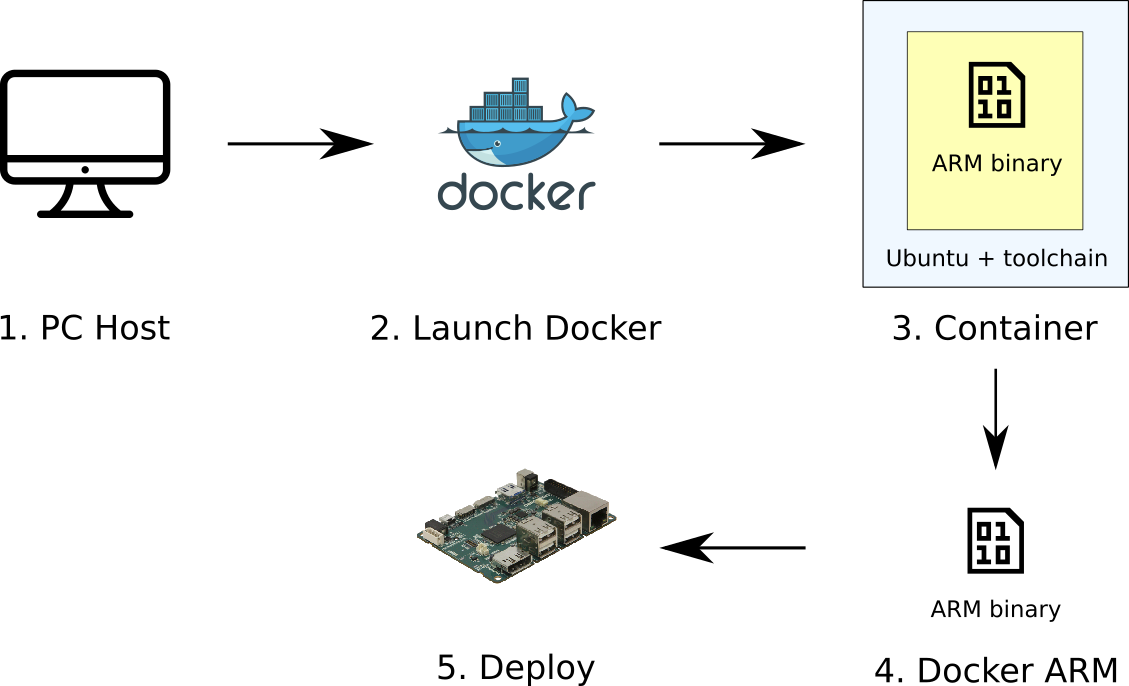
\includegraphics[scale=0.5]{img/docker_in_docker}
    \end{center}
    \caption{Docker in Docker}
    \label{fig_docker_in_docker}
\end{figure}

\subsection{Limitations}\label{maniere_officielle_limitations}

Actuellement, il est possible de générer un binaire Docker x64 et ARM mais seule l'architecture x64 intègre le \emph{deamon} nécessaire à la création de containers.

Le binaire ARM est dit \code{CLIENT\_ONLY} dans le sens où il peut être le client d'un \emph{deamon} Docker remote (instancié sur une autre machine).


\section{Compiler directement sur une machine ARM en utilisant la manière officielle}

Même principe que la technique précédente à la différence que le PC Host est remplacé par la cible, une carte ARM. On va donc avoir besoin d'une carte qui propose une distribution GNU/Linux qui intègre Docker. Dans le cas de l'Odroid XU3, il existe Archlinux ARM\footnote{Archlinux ARM: \url{https://archlinuxarm.org/}}.

\subsection{Principe utilisé}

Voir section \ref{maniere_officielle}.

Remarque: dans ce cas, seul \code{make binary} est nécessaire car on n'est pas obligé de cross compiler pour d'autres plateformes.

\subsection{Cheminement général}

Voir section \ref{maniere_officielle}.
\subsection{Schéma}

Voir section \ref{maniere_officielle}.

\subsection{Limitations}

Lors de mes tests, j'ai tenté à plusieurs reprises de compiler Docker en utilisant mon Odroid C1 personnel mais je ne suis jamais arrivé à finir la compilation car elle plantait au bout d'une bonne heure.

Évidemment, le temps de compilation est énormément long et on est limité par la machine avec laquelle on compile. Une autre possibilité pour l'avenir serait de passer par un prestataire Cloud qui fournit des machines ARM. Scaleway semble proposer ce genre d'offre\footnote{Scaleway: \url{https://www.scaleway.com/}}


\section{Compiler en émulant une machine ARM sur un PC de bureau avec QEMU et une image Debian}

\subsection{Principe utilisé}

Cette technique (et les suivantes basées sur celle-ci) est différente. Ici, on utilise une machine virtuelle QEMU\footnote{QEMU, émuler une machine complète: \url{http://wiki.qemu.org/Main_Page}} pour compiler Docker. On ne fait donc plus de cross compilation mais de l'émulation. On verra dans au chapitre \ref{executer_containers_arm_sur_x64} que l'on peut utiliser QEMU pour exécuter des containers ARM sur une machine x64.

\subsection{Cheminement général}

Il faut d'abord installer QEMU sur une machine. J'utilise Archlinux mais cela devrait être sensiblement la même chose pour d'autres distributions.

\label{install_qemu_arch}
\begin{bashcode}
yaourt -S qemu qemu-arch-extra
\end{bashcode}

Pour la suite, j'ai suivi les tutoriels suivants: 
\begin{enumerate}
\item A QEMU image for debian armel, \url{http://www.n0nb.us/blog/2012/03/a-qemu-image-for-debian-armel/}.
\item Debian Wheezy armhf images for QEMU, \url{https://people.debian.org/~aurel32/qemu/armhf/}
\end{enumerate}

Je vais pas m'étendre sur cette solution, car Debian ARM ne propose pas de package Docker et cette VM Debian ne permet pas dans sa configuration actuelle d'exécuter le binaire ARM proposé à la section \ref{binaire_arm}.

\subsection{Schéma}

Comme on peut le voir à la figure \ref{fig_docker_qemu}, on reprend le même principe qu'expliqué à la section: \nameref{maniere_officielle}.

\begin{figure}[H]
    \begin{center}
        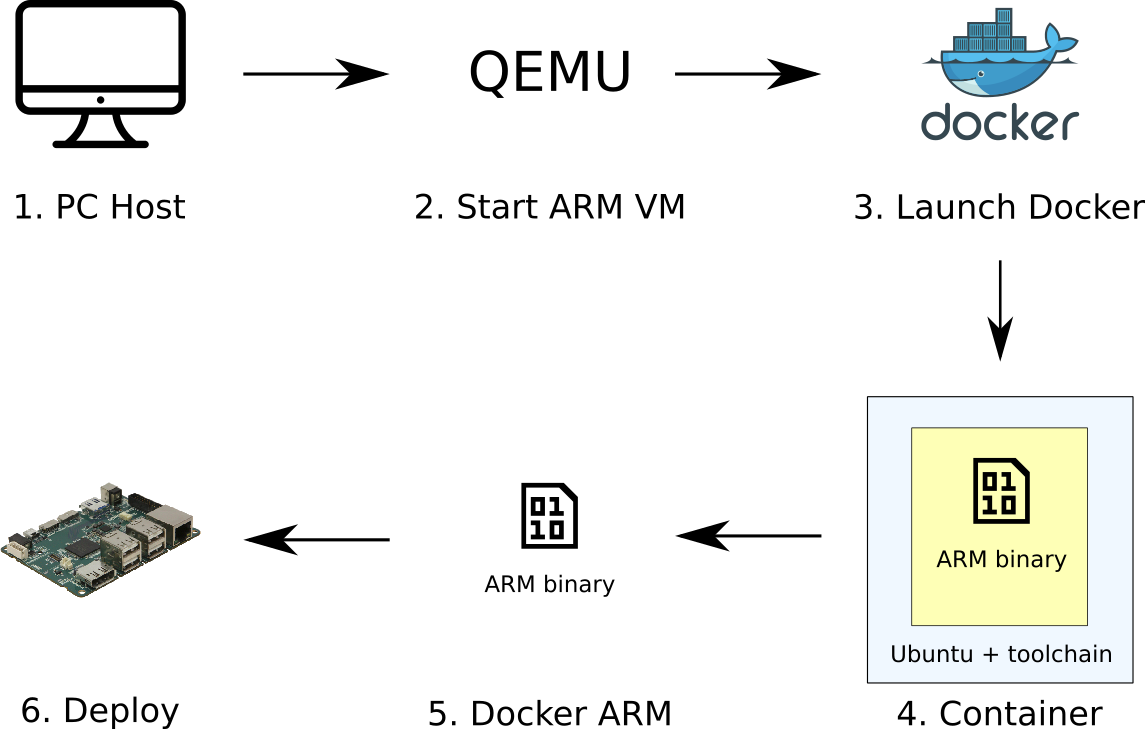
\includegraphics[scale=0.5]{img/docker_qemu}
    \end{center}
    \caption{Docker QEMU}
    \label{fig_docker_qemu}
\end{figure}

La principale différence vient du fait qu'on encapsule le processus dans une machine virtuelle QEMU afin d'éviter d'utiliser une carte ARM. Une fois le système émulé, on lance Docker pour compiler Docker.

\subsection{Limitations}

Cette solution n'est pas une solution à suivre. C'est, à mon avis, une bonne idée mais inutilisable comme présenté ici. Par contre, cela peut devenir intéressant avec d'autres distributions qui intègre un package Docker et dont le kernel est correctement configuré. Par exemple, Raspbian (Une Debian modifiée pour les Raspberry Pi) ou Archlinux ARM. Les solutions suivantes reprennent cette hypothèse\label{hypothese_debian}.


Autre point négatif, cette solution (et les dérivées utilisant QEMU) nécessite de disposer d'un binaire ARM Docker, celui de la section \ref{binaire_arm}. Par conséquent, comme on ne sait pas comment produire ce binaire, on ne maîtrise pas l'ensemble de la pipeline de compilation.


\section{Compiler en émulant une machine ARM sur un PC de bureau avec QEMU et une image Raspbian}

\subsection{Principe utilisé}

Même principe que la technique précédente à la différence près que l'image de la VM n'est plus une Debian mais une Raspbian\footnote{Raspbian: \url{https://www.raspbian.org}}, utilisée par les Raspberry Pi.

\subsection{Cheminement général}

Les étapes sont relativement les mêmes que pour la technique précédente. C'est principalement les fichiers à télécharger qui diffèrent.

Voici les tutoriels que j'ai suivis:

\begin{enumerate}
\item Émuler le Raspberry Pi sous Debian avec Qemu, \url{http://www.jdhp.org/hevea/tutoriel_rpi_qemu/tutoriel_rpi_qemu.html}
\item Émuler une Raspberry Pi sous Linux avec Qemu, \url{https://assos.centrale-marseille.fr/clubrobot/content/%C3%A9muler-une-raspberry-pi-sous-linux-avec-qemu}
\end{enumerate}

\subsection{Schéma}

Similaire à la technique précédente.

\subsection{Limitations}

Similaires à la technique précédente.

Conclusion: aucune amélioration par rapport à la technique précédente. Impossible de compiler Docker.



\section{Compiler en émulant une machine ARM sur un PC de bureau avec QEMU et chroot}

\subsection{Principe utilisé}

On va utiliser la commande \code{chroot}\footnote{chroot: \url{https://fr.wikipedia.org/wiki/Chroot}} afin d'isoler une machine QEMU dans un répertoire de notre machine de bureau.

\subsection{Cheminement général}

Le tutoriel utilisé est le suivant: \url{https://github.com/RoEdAl/linux-raspberrypi-wsp/wiki/Building-ArchLinux-ARM-packages-ona-a-PC-using-QEMU-Chroot}. Une copie de ces commandes se trouvent à l'Appendix \ref{archlinux_arm_qemu_chroot}.

\subsection{Schéma}

Comme on peut le voir à la figure \ref{fig_chroot_qemu}, la première couche représente le dossier \textit{root} de notre machine et le niveau suivant, les dossiers qu'il contient. Dans un dossier (à créer) appelé \textit{docker\_qemu}, on retrouve les fichiers utilisés par le tutoriel évoqué à la section précédente.

Dans le répertoire \textit{archlinux\_rpi2}, on retrouve le système Archlinux ARM extrait dans lequel on vient copier \code{qemu-arm-static} permettant d'émuler le système ARM.

En clair, tous les dossiers en dessus de \textit{archlinux\_rpi2} appartiennent à l'OS hôte et tous les fichiers en dessous, appartiennent au système invité, Archlinux ARM.

\begin{figure}[H]
\begin{center}
        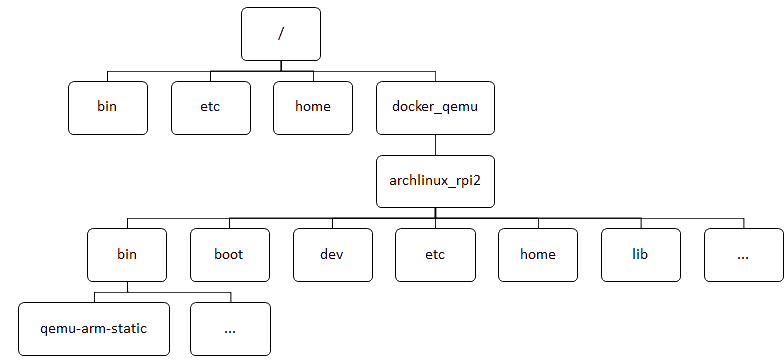
\includegraphics[scale=0.6]{img/chroot_archlinux_rpi}
        \caption{Docker QEMU}
        \label{fig_chroot_qemu}
    \end{center}
\end{figure}


\subsection{Limitations}

Bien que je sois parvenu à booter sur la machine virtuelle, je n'ai pas pu lancer la compilation de Docker car cette procédure à "détecté" que je me trouvais en \code{chroot} et s'est arrêtée.

\section{Compiler Docker sans Docker}

Avec cette technique, on essaie de court-circuiter la compilation officielle (Docker in Docker) en compilant Docker sans Docker. Pour ce faire, il faut veiller à avoir une machine qui puisse compiler Go, car Docker est écrit dans ce langage.

\textbf{Attention}: J'ai d'abord essayé de compiler Docker pour une machine x64. Cette technique était avant tout exploratoire et ne permet donc pas de compiler un binaire ARM.

\subsection{Principe utilisé}

On compile le programme de manière "classique" sans passer par un container Docker.

\subsection{Cheminement général}

Installation de Go sur Archlinux:

\begin{bashcode}
yaourt -S go
\end{bashcode}

Ensuite, on effectue les commandes suivantes:

\begin{bashcode}
git clone https://github.com/docker/docker docker_tmp
export AUTO_GOPATH=1
cd docker_tmp
git checkout v1.10.3 -b gary

# parmis les pré-requis, il manquait btrfs-progs
yaourt btrfs-progs

# on ignore devicemapper, car il y avait des erreurs.
export DOCKER_BUILDTAGS='exclude_graphdriver_devicemapper'
./hack/make.sh binary
# le binaire se trouve dans ./bundles/1.10.3/binary
\end{bashcode}

\subsection{Schéma}

\begin{figure}[H]
    \begin{center}
        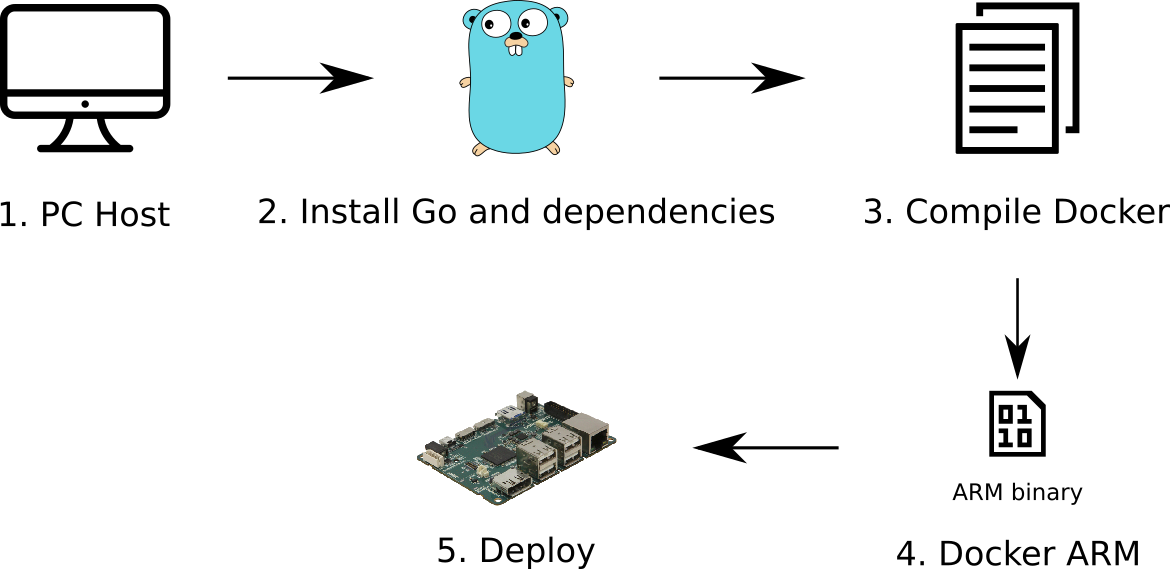
\includegraphics[scale=0.6]{img/docker_without_docker}
    \end{center}
    \caption{Docker sans Docker}
    \label{fig_docker_without_docker}
\end{figure}

La figure \ref{fig_docker_without_docker} montre la différence par rapport à la manière officielle. En effet, Docker n'est plus utilisé mais uniquement ses sources.

\subsection{Limitations}

Cette technique n'est pas une bonne idée pour les raisons suivantes:

\begin{itemize}
\item Il faut installer et configurer soit même les outils de compilations alors qu'avec la manière officielle, c'est automatiquement fait dans un container.
\item Lors de mes tests, je n'ai pas essayé de cross compiler vers ARM. C'est possible mais je ne l'ai pas testé.
\item Cette solution n'apporte rien de plus par rapport à la manière officielle. C'est-à-dire qu'elle produit (ou produirait dans le cas d'une cross compilation ARM) le même binaire qu'avec la manière officielle. Donc, le \textit{deamon} ne serait de toute façon pas disponible.

\end{itemize}

Néanmoins, cette solution m'a permis de comprendre qu'il fallait peut-être modifier le code source de Docker afin d'autoriser l'intégration du \textit{deamon} tout en conservant la technique "Docker in Docker" afin de se faciliter la vie pour installer les outils de compilation.

\section{Conclusion sur les techniques de compilation}

Comme on a pu le voir, plusieurs techniques et tentatives ont été essayées. Aucune n'a permis de  compiler ou de cross compiler Docker pour obtenir un binaire ARM statiquement lié.

Néanmoins, on sait que c'est possible car d'une part des distributions comme Archlinux ARM intègrent un package Docker incluant le \textit{deamon} et d'une autre car on a pu mettre la main sur un binaire isolé, voir section \ref{binaire_arm}.

Encore une fois, il n'est pas impossible que l'équipe Docker supporte officiellement le \textit{deamon} pour la plateforme ARM d'ici quelques temps et ce document sera obsolète.

Pour la suite du projet, j'ai installé Archlinux ARM sur l'Odroid XU3 et vais continuer avec une partie concernant la sécurité de Docker et de ces containers.

\chapter{Exécuter des containers ARM sur une machine x64}\label{executer_containers_arm_sur_x64}

Dans ce chapitre, on va voir comment exécuter des containers basés sur des images ARM sur une machine x64. Ceci permet plusieurs choses intéressantes comme:

\begin{itemize}
\item Tester une image sur son poste avant de la déployer sur une cible
\item Pouvoir utiliser des images prévues pour ARM sur une machine x64, voire d'en effectuer le portage
\item Utiliser le container ARM comme outil de cross compilation
\item Pouvoir développer une application ARM et la tester sur le même PC sans devoir la déployer sur la cible à chaque compilation
\item ...
\end{itemize}


Lien utile : \url{http://blog.hypriot.com/post/close-encounters-of-the-third-kind/}

On va reprendre l'exemple du blog de Hypriot et lancer un container httpd ARM (un serveur web et une page HTML toute simple).

Il faut d'abord installer QEMU. Pour ce faire, voir section \ref{install_qemu_arch}.

Ensuite, il faut créer un Dockerfile qui se base sur l'image ARM (ici \code{hypriot/rpi-busybox-httpd}) à lancer et une archive contenant \code{qemu-static-arm}.

Création d'un dossier de travail:

\begin{bashcode}
mkdir hypriot-qemu
cd hypriot-qemu
touch Dockerfile
\end{bashcode}

Dockerfile à créer sur une machine x64:

\begin{bashcode}
FROM hypriot/rpi-busybox-httpd
ADD qemu-arm-static.tar /
\end{bashcode}

Pour l'archive, il faut effectuer les manipulations suivantes :

\begin{bashcode}
sudo cp /usr/bin/qemu-arm-static .
sudo chown gary:gary qemu-arm-static
mkdir usr
tar -cvf qemu-arm-static.tar usr
mkdir usr/bin
tar -uvf qemu-arm-static.tar usr/bin
mv qemu-arm-static usr/bin
tar -uvf qemu-arm-static.tar usr/bin/qemu-arm-static
\end{bashcode}

Si tout s'est bien passé, vous devriez obtenir une sortie similaire :

\begin{bashcode}
tar vtf qemu-arm-static.tar
drwxrwxr-x gary/gary         0 2016-04-15 21:35 usr/
drwxrwxr-x gary/gary         0 2016-04-15 21:35 usr/bin/
-rwxr-xr-x gary/gary   2936324 2016-04-15 21:26 usr/bin/qemu-arm-static
\end{bashcode}

Il ne reste plus qu'à lancer le container :

\begin{bashcode}
docker build -t rpi-busybox-httpd .
docker run -d -p 80:80 rpi-busybox-httpd # essayez un autre port s'il est déjà pris
\end{bashcode}

Rendez-vous ensuite sur \url{http://localhost:80} pour observer la page web.

\begin{appendices}
  \chapter{Script : Write system on SD}\label{write_system_sd}

  \inputminted[xleftmargin=20pt, linenos=true, breaklines=true, frame=single, framesep=6pt, tabsize=2, fontfamily=courier, fontsize=\small]{bash}{../write_system_on_sd.sh}
  
  \chapter{Building ArchLinux ARM packages on a PC using QEMU Chroot}\label{archlinux_arm_qemu_chroot}
  
\textbf{Source}: \url{https://github.com/RoEdAl/linux-raspberrypi-wsp/wiki/Building-ArchLinux-ARM-packages-ona-a-PC-using-QEMU-Chroot}

On a PC witch ArchLinux or Manjaro installed:

Build and install binfmt-support package.
Build and install qemu-user-static package.
Install arch-install-scripts package.

Download and extract the root filesystem for Raspberry Pi or Raspberry Pi 2:

\begin{bashcode}
wget http://archlinuxarm.org/os/ArchLinuxARM-rpi-latest.tar.gz   
bsdtar -xpf ArchLinuxARM-rpi-latest.tar.gz -C archlinux-rpi
\end{bashcode}

or

\begin{bashcode}
wget http://archlinuxarm.org/os/ArchLinuxARM-rpi-2-latest.tar.gz   
bsdtar -xpf ArchLinuxARM-rpi-2-latest.tar.gz -C archlinux-rpi2
\end{bashcode}

Enable ARM to x86 translation:

\begin{bashcode}    
update-binfmts --enable qemu-arm
\end{bashcode}


Copy the \textbf{QEMU} executable:

\begin{bashcode}
cp /usr/bin/qemu-arm-static archlinux-rpi/usr/bin
\end{bashcode}


Chroot:

\begin{bashcode}
arch-chroot archlinux-rpi /bin/bash
\end{bashcode}


Install base-devel and distcc packages:

\begin{bashcode}
pacman -Suy base-devel distcc
\end{bashcode}


Exit and chroot again as normal alarm user:

\begin{bashcode}
exit
arch-chroot archlinux-rpi runuser -l alarm
\end{bashcode}


Build your package.

\end{appendices}
\end{document}
